\documentclass[]{article}
\usepackage{lmodern}
\usepackage{amssymb,amsmath}
\usepackage{ifxetex,ifluatex}
\usepackage{fixltx2e} % provides \textsubscript
\ifnum 0\ifxetex 1\fi\ifluatex 1\fi=0 % if pdftex
  \usepackage[T1]{fontenc}
  \usepackage[utf8]{inputenc}
\else % if luatex or xelatex
  \ifxetex
    \usepackage{mathspec}
  \else
    \usepackage{fontspec}
  \fi
  \defaultfontfeatures{Ligatures=TeX,Scale=MatchLowercase}
\fi
% use upquote if available, for straight quotes in verbatim environments
\IfFileExists{upquote.sty}{\usepackage{upquote}}{}
% use microtype if available
\IfFileExists{microtype.sty}{%
\usepackage{microtype}
\UseMicrotypeSet[protrusion]{basicmath} % disable protrusion for tt fonts
}{}
\usepackage[margin=1in]{geometry}
\usepackage{hyperref}
\hypersetup{unicode=true,
            pdftitle={naniar: Expanding ggplot2 for better visual exploration missingsness},
            pdfauthor={Nicholas Tierney, Di Cook},
            pdfborder={0 0 0},
            breaklinks=true}
\urlstyle{same}  % don't use monospace font for urls
\usepackage{color}
\usepackage{fancyvrb}
\newcommand{\VerbBar}{|}
\newcommand{\VERB}{\Verb[commandchars=\\\{\}]}
\DefineVerbatimEnvironment{Highlighting}{Verbatim}{commandchars=\\\{\}}
% Add ',fontsize=\small' for more characters per line
\usepackage{framed}
\definecolor{shadecolor}{RGB}{248,248,248}
\newenvironment{Shaded}{\begin{snugshade}}{\end{snugshade}}
\newcommand{\KeywordTok}[1]{\textcolor[rgb]{0.13,0.29,0.53}{\textbf{{#1}}}}
\newcommand{\DataTypeTok}[1]{\textcolor[rgb]{0.13,0.29,0.53}{{#1}}}
\newcommand{\DecValTok}[1]{\textcolor[rgb]{0.00,0.00,0.81}{{#1}}}
\newcommand{\BaseNTok}[1]{\textcolor[rgb]{0.00,0.00,0.81}{{#1}}}
\newcommand{\FloatTok}[1]{\textcolor[rgb]{0.00,0.00,0.81}{{#1}}}
\newcommand{\ConstantTok}[1]{\textcolor[rgb]{0.00,0.00,0.00}{{#1}}}
\newcommand{\CharTok}[1]{\textcolor[rgb]{0.31,0.60,0.02}{{#1}}}
\newcommand{\SpecialCharTok}[1]{\textcolor[rgb]{0.00,0.00,0.00}{{#1}}}
\newcommand{\StringTok}[1]{\textcolor[rgb]{0.31,0.60,0.02}{{#1}}}
\newcommand{\VerbatimStringTok}[1]{\textcolor[rgb]{0.31,0.60,0.02}{{#1}}}
\newcommand{\SpecialStringTok}[1]{\textcolor[rgb]{0.31,0.60,0.02}{{#1}}}
\newcommand{\ImportTok}[1]{{#1}}
\newcommand{\CommentTok}[1]{\textcolor[rgb]{0.56,0.35,0.01}{\textit{{#1}}}}
\newcommand{\DocumentationTok}[1]{\textcolor[rgb]{0.56,0.35,0.01}{\textbf{\textit{{#1}}}}}
\newcommand{\AnnotationTok}[1]{\textcolor[rgb]{0.56,0.35,0.01}{\textbf{\textit{{#1}}}}}
\newcommand{\CommentVarTok}[1]{\textcolor[rgb]{0.56,0.35,0.01}{\textbf{\textit{{#1}}}}}
\newcommand{\OtherTok}[1]{\textcolor[rgb]{0.56,0.35,0.01}{{#1}}}
\newcommand{\FunctionTok}[1]{\textcolor[rgb]{0.00,0.00,0.00}{{#1}}}
\newcommand{\VariableTok}[1]{\textcolor[rgb]{0.00,0.00,0.00}{{#1}}}
\newcommand{\ControlFlowTok}[1]{\textcolor[rgb]{0.13,0.29,0.53}{\textbf{{#1}}}}
\newcommand{\OperatorTok}[1]{\textcolor[rgb]{0.81,0.36,0.00}{\textbf{{#1}}}}
\newcommand{\BuiltInTok}[1]{{#1}}
\newcommand{\ExtensionTok}[1]{{#1}}
\newcommand{\PreprocessorTok}[1]{\textcolor[rgb]{0.56,0.35,0.01}{\textit{{#1}}}}
\newcommand{\AttributeTok}[1]{\textcolor[rgb]{0.77,0.63,0.00}{{#1}}}
\newcommand{\RegionMarkerTok}[1]{{#1}}
\newcommand{\InformationTok}[1]{\textcolor[rgb]{0.56,0.35,0.01}{\textbf{\textit{{#1}}}}}
\newcommand{\WarningTok}[1]{\textcolor[rgb]{0.56,0.35,0.01}{\textbf{\textit{{#1}}}}}
\newcommand{\AlertTok}[1]{\textcolor[rgb]{0.94,0.16,0.16}{{#1}}}
\newcommand{\ErrorTok}[1]{\textcolor[rgb]{0.64,0.00,0.00}{\textbf{{#1}}}}
\newcommand{\NormalTok}[1]{{#1}}
\usepackage{longtable,booktabs}
\usepackage{graphicx,grffile}
\makeatletter
\def\maxwidth{\ifdim\Gin@nat@width>\linewidth\linewidth\else\Gin@nat@width\fi}
\def\maxheight{\ifdim\Gin@nat@height>\textheight\textheight\else\Gin@nat@height\fi}
\makeatother
% Scale images if necessary, so that they will not overflow the page
% margins by default, and it is still possible to overwrite the defaults
% using explicit options in \includegraphics[width, height, ...]{}
\setkeys{Gin}{width=\maxwidth,height=\maxheight,keepaspectratio}
\IfFileExists{parskip.sty}{%
\usepackage{parskip}
}{% else
\setlength{\parindent}{0pt}
\setlength{\parskip}{6pt plus 2pt minus 1pt}
}
\setlength{\emergencystretch}{3em}  % prevent overfull lines
\providecommand{\tightlist}{%
  \setlength{\itemsep}{0pt}\setlength{\parskip}{0pt}}
\setcounter{secnumdepth}{0}
% Redefines (sub)paragraphs to behave more like sections
\ifx\paragraph\undefined\else
\let\oldparagraph\paragraph
\renewcommand{\paragraph}[1]{\oldparagraph{#1}\mbox{}}
\fi
\ifx\subparagraph\undefined\else
\let\oldsubparagraph\subparagraph
\renewcommand{\subparagraph}[1]{\oldsubparagraph{#1}\mbox{}}
\fi

%%% Use protect on footnotes to avoid problems with footnotes in titles
\let\rmarkdownfootnote\footnote%
\def\footnote{\protect\rmarkdownfootnote}

%%% Change title format to be more compact
\usepackage{titling}

% Create subtitle command for use in maketitle
\newcommand{\subtitle}[1]{
  \posttitle{
    \begin{center}\large#1\end{center}
    }
}

\setlength{\droptitle}{-2em}
  \title{naniar: Expanding ggplot2 for better visual exploration missingsness}
  \pretitle{\vspace{\droptitle}\centering\huge}
  \posttitle{\par}
  \author{Nicholas Tierney, Di Cook}
  \preauthor{\centering\large\emph}
  \postauthor{\par}
  \predate{\centering\large\emph}
  \postdate{\par}
  \date{14/12/2016}


\begin{document}
\maketitle

\section{Introduction}\label{introduction}

Missing data is ubiquitous in data analysis, and are often the source of
much energy, frustration, and confusion. Since 2014 there has been
substantial development in the area of ``tidy data'' {[} @wickham{]},
which states the (surprisingly simple!) rule that each row is an
observation and each column is a variable, which makes it easy to reason
with data. This paper describes approaches for summarising missing data
in numerical and graphical forms whilst maintaining a tidy format.

\section{Types of missing data}\label{types-of-missing-data}

Canonical sources of missing data are questionnaires. Data obtained from
questionnaires are often subject to both unknown and known missingness
structure. For example, unknown missing data structure can arise from
respondents accidentally failing to answer questions or inadvertently
providing inappropriate answers. Known missing data structure data may
arise due to the structure of the questionnaire. For example, the first
question on a survey might be: `If YES, skip to question 4', resulting
in questions 2 and 3 missing. If the structure of the questionnaire is
known, this type of missingness can be evaluated easily. However, if
this information is not available, the mechanism responsible for
producing missing data must be inferred from the data.

Another common source of known and unknown structured missingness is
medical examination data. The results of particular medical tests may
be: missing for purely random reasons, missing due to the procedure, or
missing based on decisions arising from the observed data. For example,
a young patient is young may not be subjected to neurodegenerative tests
reserved for older workers. A final example is dropouts in a
longitudinal study, where participants do not return for future testing
sessions. In this case, it is difficult, sometimes impossible, to
ascertain the reason for the dropouts, and hence, whether the
missingness structure. However, this ascertainment is essential if the
estimates based on these data are to be believed as unbiased,
{[}@Simon1986; @Little1988; @Rubin1976{]}.

Other categories of missing data are sometimes identified: Missing
Completeley at Random (MCAR), Missing At Random (MAR), and Missing Not
At Random (MNAR) {[} @Little2002{]}. MCAR describes where missingness
has no association with the observed or unobserved data. MAR describes
cases where missingness depends on data observed, but not data
unobserved. MNAR is where the missingness of the response is related to
an unobserved value relevant to the assessment of interest.

XXX How have you met missings before? What examples of data were you
working with that had missing value problems?

\subsection{Existing packages for handling missing
data}\label{existing-packages-for-handling-missing-data}

XXX Describe exisiting packages, and group them into what they do

Software focussing on missing data typically focus on imputation or
visualisation. Imputation packages such as mice, Hmisc, mi, Amelia, and
mitools provide functions to facilitate imputation, aggregation of
imputations, diagnostics, and define user-written imputation functions
{[}@mice; @Hmisc; etc. {]}. It is important to remember that care must
be taken to avoid bias when performing multiple imputation.

Missing data visualisation packages include the R package VIM, and the
stand alone softwares MANET, ggobi, and MissingDataGUI.

MANET (Missings Are Now Equally Treated), provides univariate
visualisations of missing data using linked brushing, using a
referential plot to display the proportion of missingness for each
variable as a filled bar plot, and then displayed plots of the data,
using a histogram (for continuous data) or a barplot (for categorical
data). The plots of the data were highlighted when values of one
variable were in the same row as a missing value.

\emph{some sort of figure describing this?}

ggobi provided multivariate visualisation of missing data using two
methods. The first involved a reference plot providing a visual
cross-tabulation of the data according to missing or not missing. This
was then linked to a parallel coordinate plot, such that whichever
values from the reference plot were then highlighted on the parallel
coordinate plot. ggobi also provided scatterplot plots of missingness,
where the variables are \ldots{}

XXX One sentence on why MissingDataGUI is too heavy weight for general
purpose

MissingDataGUI provides a user interface for exploring missing data
structure both numerically and visually, it also provides visualisation
methods for visualising imputated values. A limitation of MissingDataGUI
is that it breaks workflow by being a separate part of analysis, where
one might be performing an analysis using R, using Also being separate
from

XXX One paragraph on how ggplot2 handles missing values (or not): a
message is printed and then the missings are ignored

ggplot2, a (very popular) package for producing elegant graphics in R,
currently only provides visualisation for missing data when there is a
category variable, this provides visualisations for missing data when
the values being plotted are categories, it treats one of the categories
as a NA value. Outside of this, ggplot2 does not provide much support
for visualisation of missing data. It currently prints out a warning
message when a plot us shown that contains missing data, which states
that it has removed a particular number of rows containing
``non-finite'' values.

See some examples below (not for the paper, but for explaining right
now:

\begin{Shaded}
\begin{Highlighting}[]
\NormalTok{data_test <-}\StringTok{ }\KeywordTok{data_frame}\NormalTok{(}\DataTypeTok{x =} \KeywordTok{c}\NormalTok{(}\DecValTok{1}\NormalTok{,}\DecValTok{2}\NormalTok{,}\DecValTok{3}\NormalTok{,}\DecValTok{4}\NormalTok{,}\DecValTok{5}\NormalTok{,}\DecValTok{5}\NormalTok{,}\DecValTok{5}\NormalTok{,}\DecValTok{5}\NormalTok{,}\OtherTok{NA}\NormalTok{,}\OtherTok{NA}\NormalTok{),}
                        \DataTypeTok{y =} \KeywordTok{c}\NormalTok{(}\DecValTok{9}\NormalTok{,}\DecValTok{5}\NormalTok{,}\DecValTok{6}\NormalTok{,}\DecValTok{7}\NormalTok{,}\DecValTok{4}\NormalTok{,}\DecValTok{9}\NormalTok{,}\DecValTok{2}\NormalTok{,}\DecValTok{4}\NormalTok{,}\DecValTok{4}\NormalTok{,}\DecValTok{5}\NormalTok{))}

  \KeywordTok{ggplot}\NormalTok{(data_test,}
         \KeywordTok{aes}\NormalTok{(}\DataTypeTok{x =} \KeywordTok{factor}\NormalTok{(x),}
             \DataTypeTok{y =} \NormalTok{y)) +}\StringTok{ }
\StringTok{  }\KeywordTok{geom_bar}\NormalTok{(}\DataTypeTok{stat =} \StringTok{"identity"}\NormalTok{)}
\end{Highlighting}
\end{Shaded}

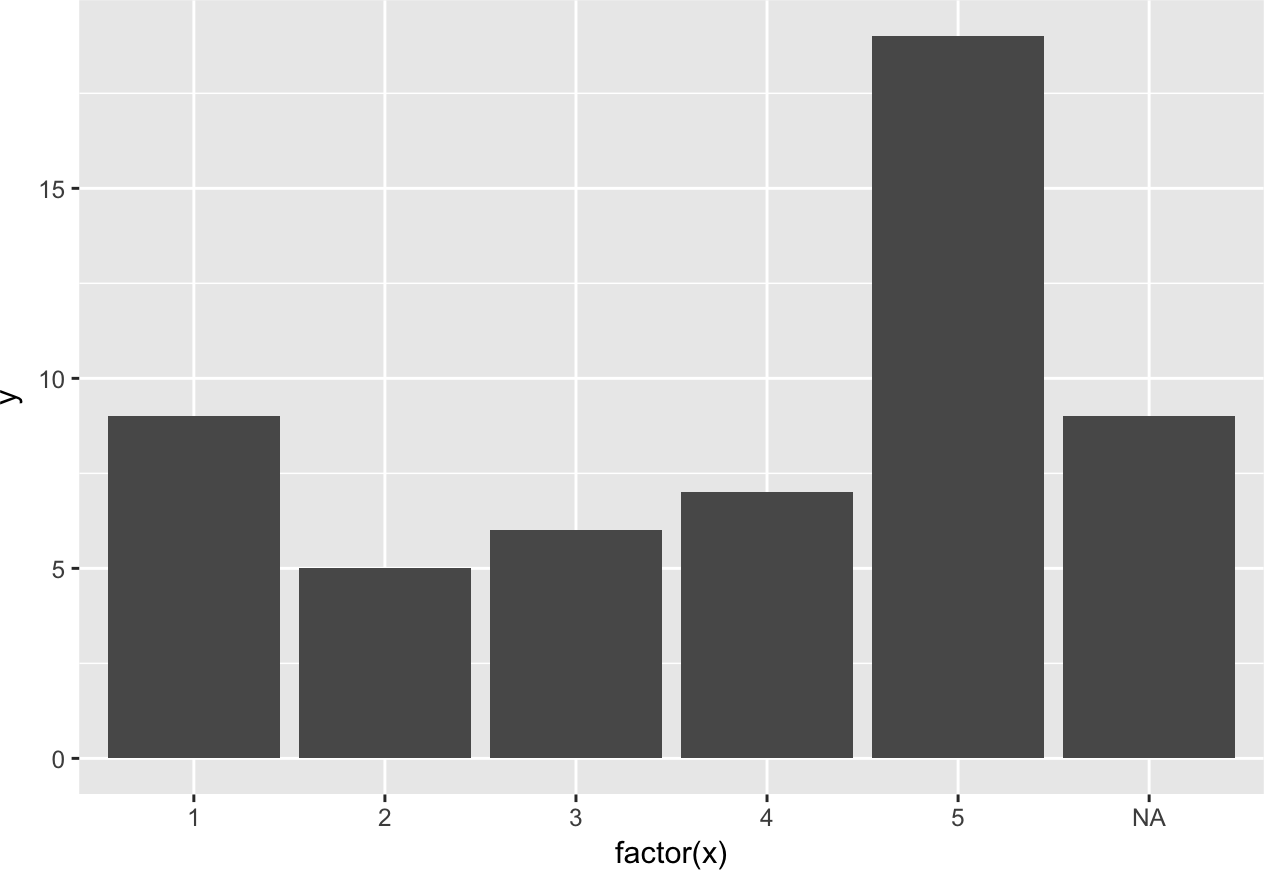
\includegraphics{jsm2017_files/figure-latex/ggplot-missing-vals-1.png}

\begin{Shaded}
\begin{Highlighting}[]
  \KeywordTok{ggplot}\NormalTok{(data_test,}
         \KeywordTok{aes}\NormalTok{(}\DataTypeTok{x =} \KeywordTok{factor}\NormalTok{(x),}
             \DataTypeTok{y =} \NormalTok{y)) +}\StringTok{ }
\StringTok{  }\KeywordTok{geom_boxplot}\NormalTok{()}
\end{Highlighting}
\end{Shaded}

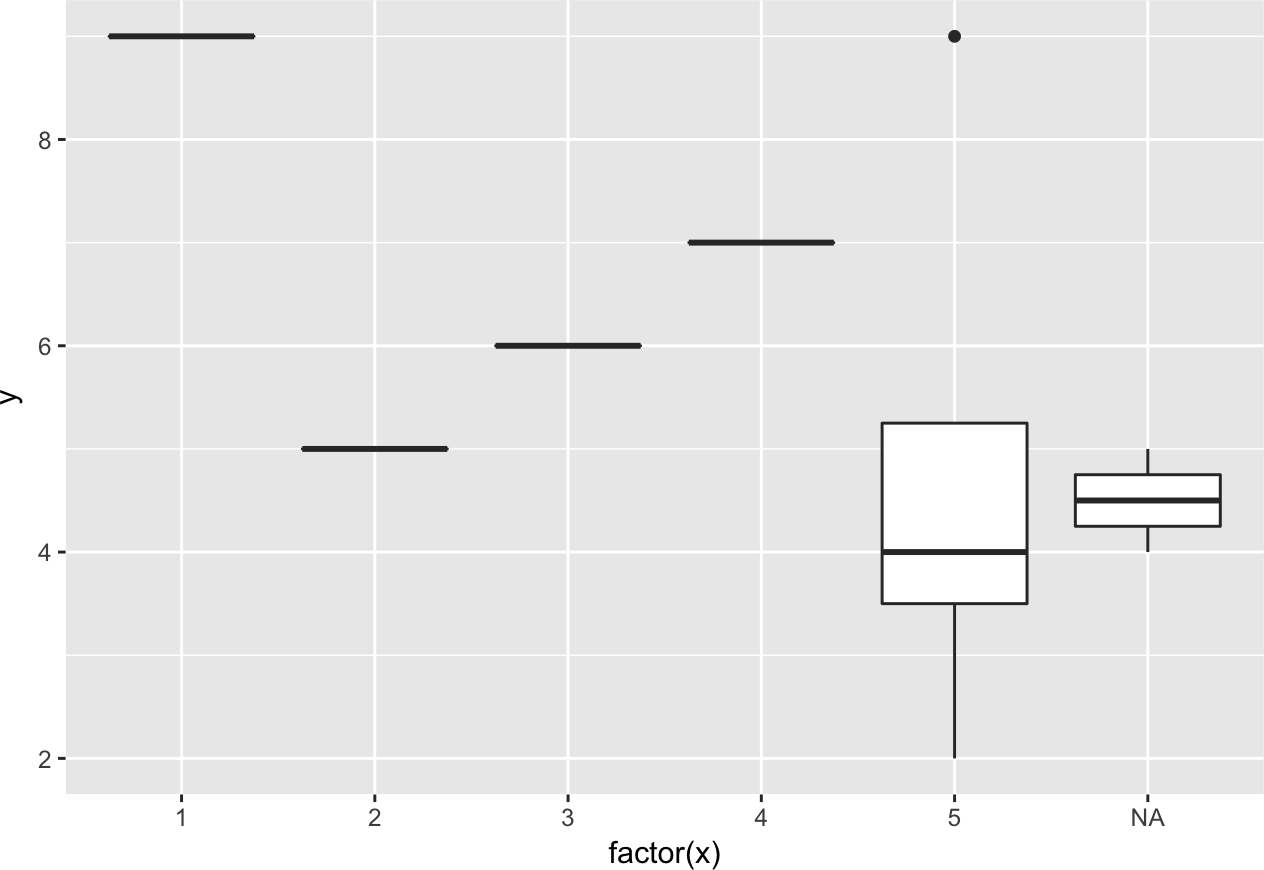
\includegraphics{jsm2017_files/figure-latex/ggplot-missing-vals-2.png}

\begin{Shaded}
\begin{Highlighting}[]
  \KeywordTok{ggplot}\NormalTok{(data_test,}
         \KeywordTok{aes}\NormalTok{(}\DataTypeTok{x =} \KeywordTok{factor}\NormalTok{(x),}
             \DataTypeTok{y =} \NormalTok{y)) +}\StringTok{ }
\StringTok{  }\KeywordTok{geom_point}\NormalTok{()}
\end{Highlighting}
\end{Shaded}

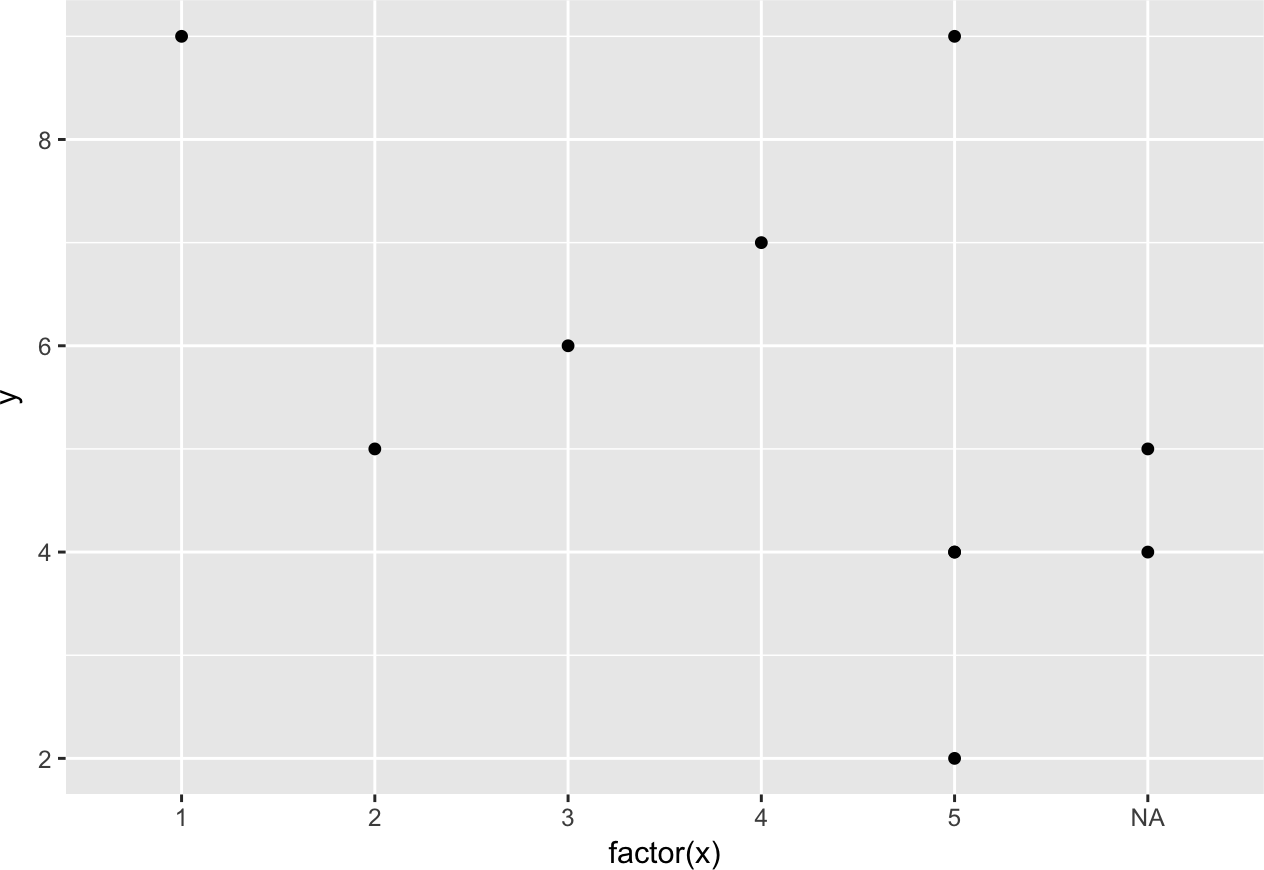
\includegraphics{jsm2017_files/figure-latex/ggplot-missing-vals-3.png}

\section{Data structures for missing
data}\label{data-structures-for-missing-data}

\begin{Shaded}
\begin{Highlighting}[]
\CommentTok{# create a simple example of missing data for the paper to illustrate the shadow matrix}
\NormalTok{df_example <-}\StringTok{  }\NormalTok{tibble::}\KeywordTok{tribble}\NormalTok{(~V1, ~V2, ~V3, ~V4,}
                               \StringTok{"A"}\NormalTok{, }\DecValTok{15}\NormalTok{, }\FloatTok{1.2}\NormalTok{, }\OtherTok{NA}\NormalTok{,}
                               \StringTok{"A"}\NormalTok{, }\OtherTok{NA}\NormalTok{, }\OtherTok{NA}\NormalTok{, T,}
                               \StringTok{"A"}\NormalTok{, }\DecValTok{18}\NormalTok{, }\OtherTok{NA}\NormalTok{, F,}
                               \StringTok{"B"}\NormalTok{, }\DecValTok{5}\NormalTok{, }\FloatTok{1.6}\NormalTok{, T,}
                               \StringTok{"B"}\NormalTok{, }\OtherTok{NA}\NormalTok{, }\FloatTok{0.7}\NormalTok{, T,}
                               \StringTok{"B"}\NormalTok{, }\DecValTok{12}\NormalTok{, }\OtherTok{NA}\NormalTok{, F)}
\end{Highlighting}
\end{Shaded}

Representing missing data structure is achieed using the shadow matrix,
introduced in Swayne and Buja {[}-@Swayne1998{]}. The shadow matrix is
the same dimension as the data, and consists of binary indicators of
``missingness'' of data values. In our case, missing is represented as
``NA'', and not missing is represented as ``!NA'', although these may be
represented as 1 and 0, respectively. This helps us explicitly describe
the missingness structure. Representing it as its own separate matrix
also helps us separate out the multivariate nature of missing data, as
different cases have missing values in different sets of variables.

\begin{figure}[htbp]
\centering
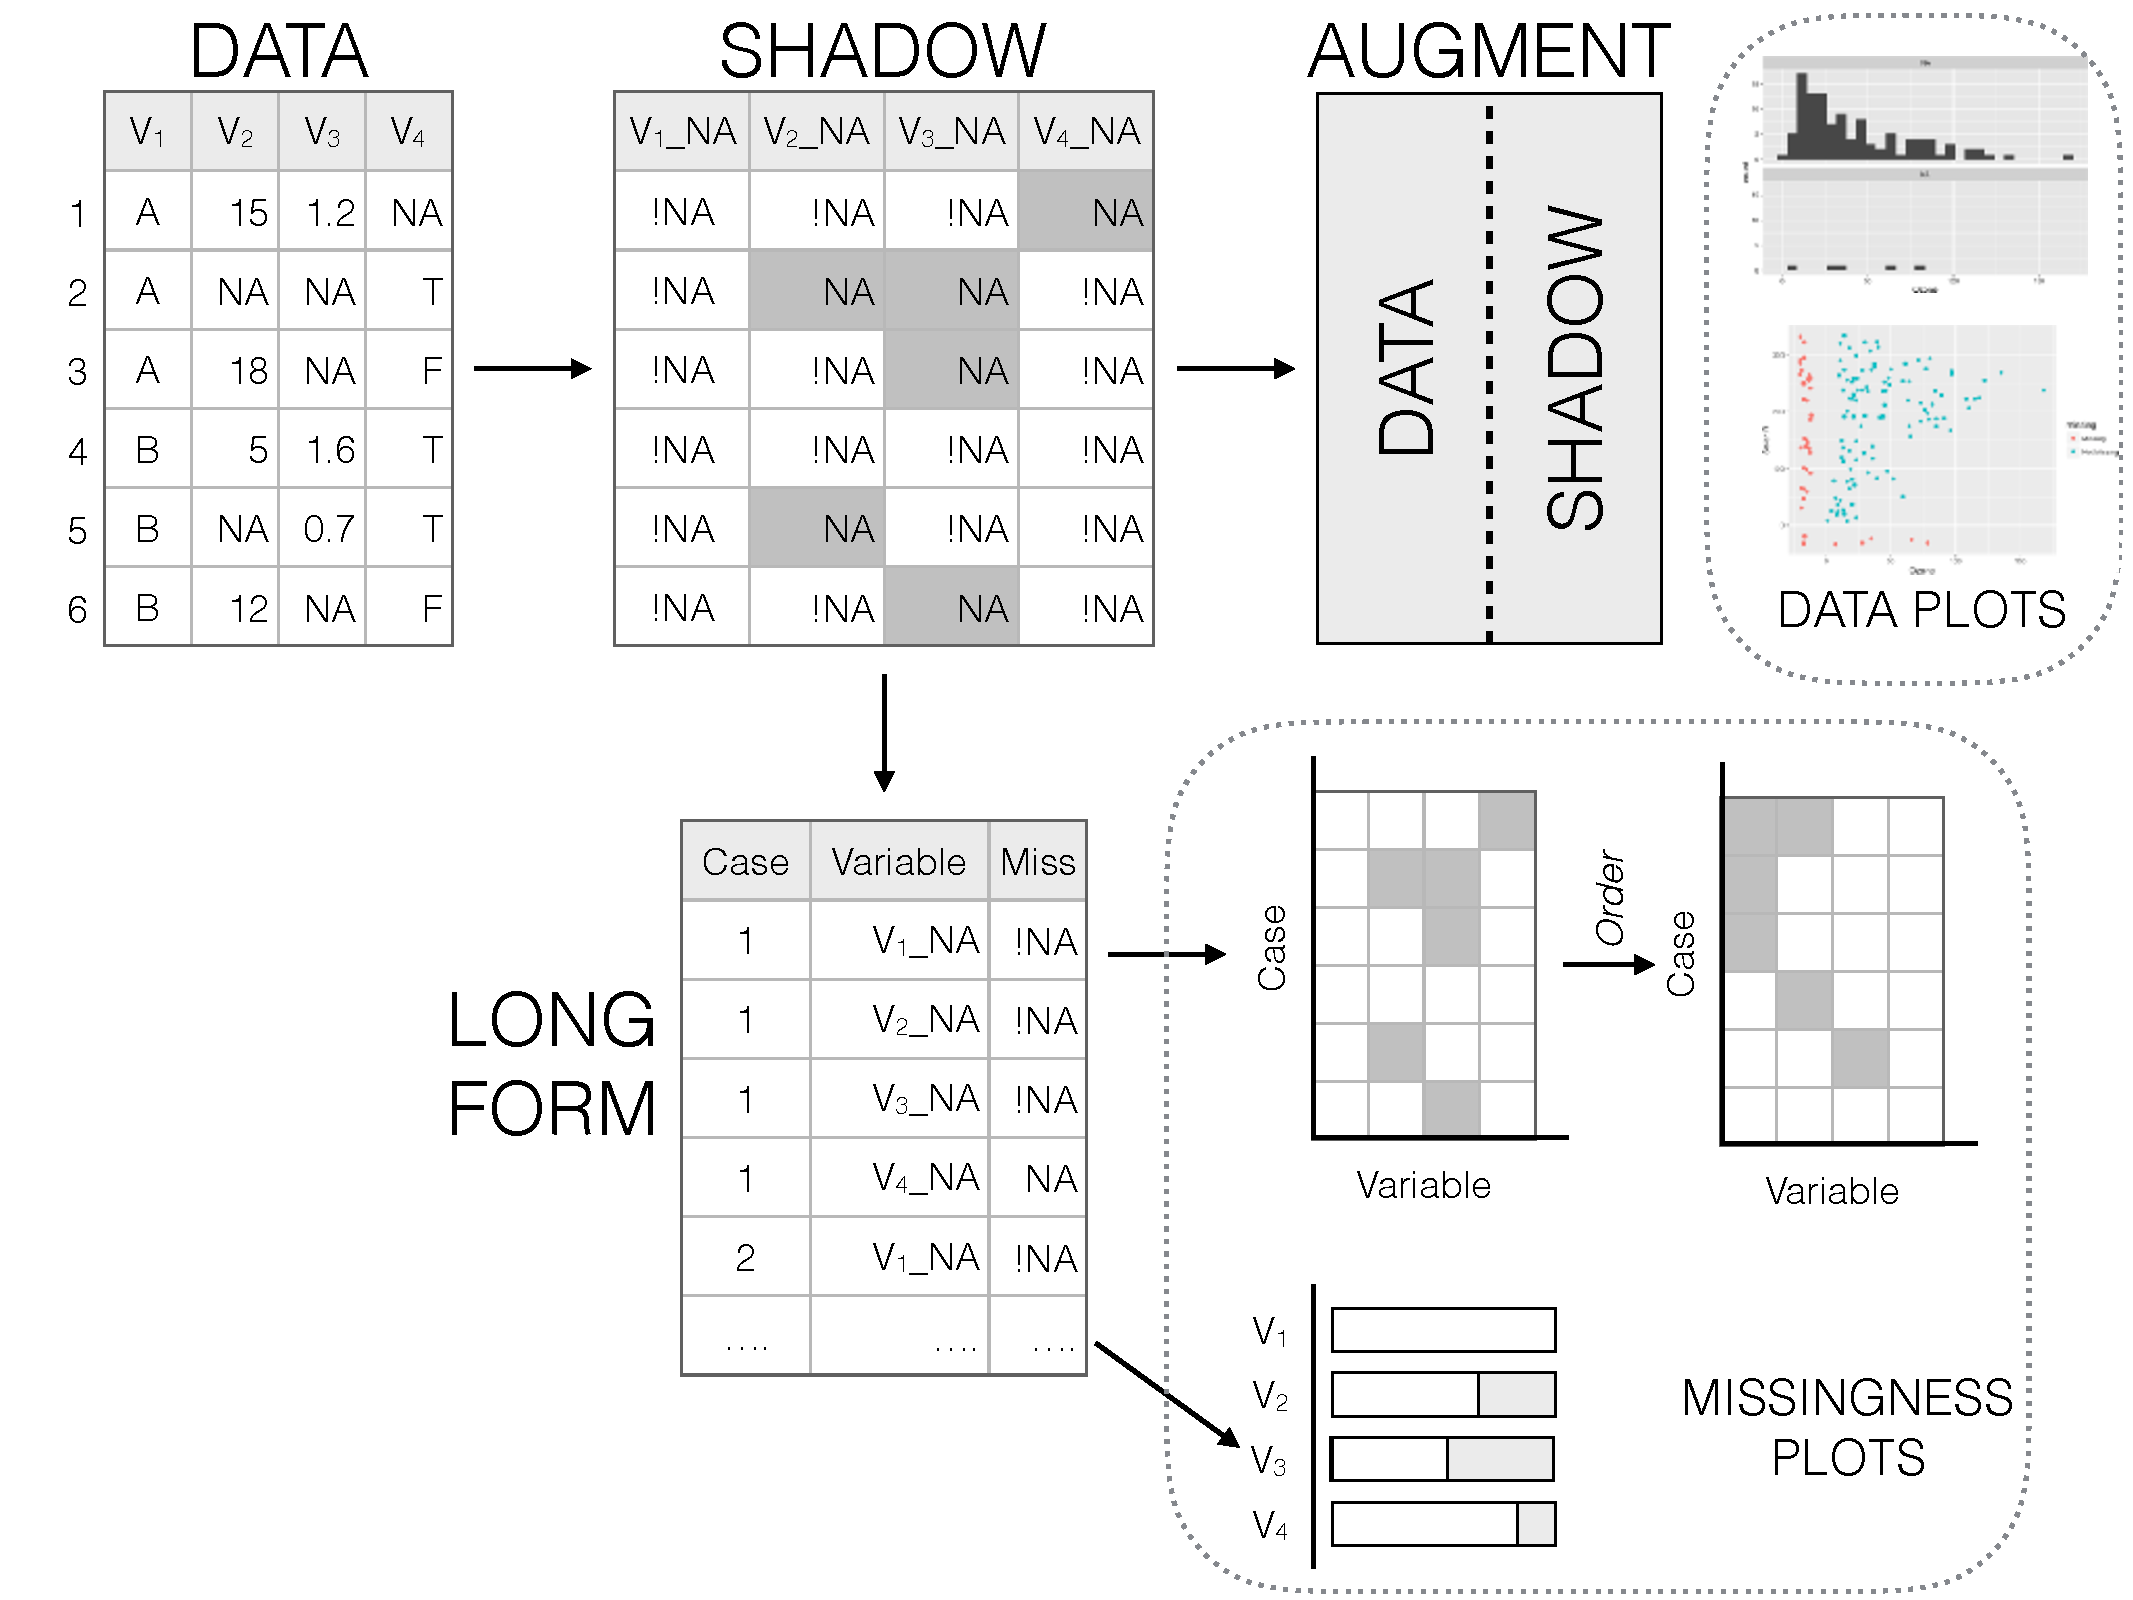
\includegraphics{/Users/tierneyn/Google Drive/ALL THE THINGS/PhD/code/R/jsm2017/diagram.pdf}
\caption{diagram of shadow missing}
\end{figure}

The shadow matrix is represented below:

\begin{longtable}[]{@{}llll@{}}
\toprule
V1\_NA & V2\_NA & V3\_NA & V4\_NA\tabularnewline
\midrule
\endhead
!NA & !NA & !NA & NA\tabularnewline
!NA & NA & NA & !NA\tabularnewline
!NA & !NA & NA & !NA\tabularnewline
!NA & !NA & !NA & !NA\tabularnewline
!NA & NA & !NA & !NA\tabularnewline
!NA & !NA & NA & !NA\tabularnewline
\bottomrule
\end{longtable}

It can also be bound in a wide format, column-wise, to the existing
datastructure, adding the suffix ``\_NA" to the data.

\begin{Shaded}
\begin{Highlighting}[]
\NormalTok{knitr::}\KeywordTok{kable}\NormalTok{(}\KeywordTok{bind_shadow}\NormalTok{(df_example))}
\end{Highlighting}
\end{Shaded}

\begin{longtable}[]{@{}lrrlllll@{}}
\toprule
V1 & V2 & V3 & V4 & V1\_NA & V2\_NA & V3\_NA & V4\_NA\tabularnewline
\midrule
\endhead
A & 15 & 1.2 & NA & !NA & !NA & !NA & NA\tabularnewline
A & NA & NA & TRUE & !NA & NA & NA & !NA\tabularnewline
A & 18 & NA & FALSE & !NA & !NA & NA & !NA\tabularnewline
B & 5 & 1.6 & TRUE & !NA & !NA & !NA & !NA\tabularnewline
B & NA & 0.7 & TRUE & !NA & NA & !NA & !NA\tabularnewline
B & 12 & NA & FALSE & !NA & !NA & NA & !NA\tabularnewline
\bottomrule
\end{longtable}

Another format is to display it in long form, as below:

\begin{Shaded}
\begin{Highlighting}[]
\KeywordTok{as_shadow}\NormalTok{(df_example) %>%}
\StringTok{  }\KeywordTok{mutate}\NormalTok{(}\DataTypeTok{rows =} \DecValTok{1}\NormalTok{:}\KeywordTok{nrow}\NormalTok{(.)) %>%}
\StringTok{  }\KeywordTok{gather}\NormalTok{(}\DataTypeTok{key =} \StringTok{"var"}\NormalTok{,}
         \DataTypeTok{value =} \StringTok{"miss"}\NormalTok{,}
         \NormalTok{-rows) %>%}
\StringTok{  }\KeywordTok{slice}\NormalTok{(}\DecValTok{1}\NormalTok{:}\DecValTok{10}\NormalTok{) %>%}
\StringTok{  }\NormalTok{knitr::}\KeywordTok{kable}\NormalTok{()}
\end{Highlighting}
\end{Shaded}

\begin{longtable}[]{@{}rll@{}}
\toprule
rows & var & miss\tabularnewline
\midrule
\endhead
1 & V1\_NA & !NA\tabularnewline
2 & V1\_NA & !NA\tabularnewline
3 & V1\_NA & !NA\tabularnewline
4 & V1\_NA & !NA\tabularnewline
5 & V1\_NA & !NA\tabularnewline
6 & V1\_NA & !NA\tabularnewline
1 & V2\_NA & !NA\tabularnewline
2 & V2\_NA & NA\tabularnewline
3 & V2\_NA & !NA\tabularnewline
4 & V2\_NA & !NA\tabularnewline
\bottomrule
\end{longtable}

\subsection{Visualisation of missing
data}\label{visualisation-of-missing-data}

\textbf{Heatmap (plot of the long form)}

One common method for visualising missing data is to display a heatmap
of the shadow matrix. This approach can be very helpful for giving an
overview of which variables contain the most missingness. Methods can
also be applied to rearrange rows and columns to find clusters, and
identify other interesting features of the data that may have previously
been hidden or unclear. This method is shown below using the
\texttt{vis\_miss} from the \texttt{visdat} package.

\begin{Shaded}
\begin{Highlighting}[]
\KeywordTok{library}\NormalTok{(visdat)}
\KeywordTok{vis_miss}\NormalTok{(airquality)}
\end{Highlighting}
\end{Shaded}

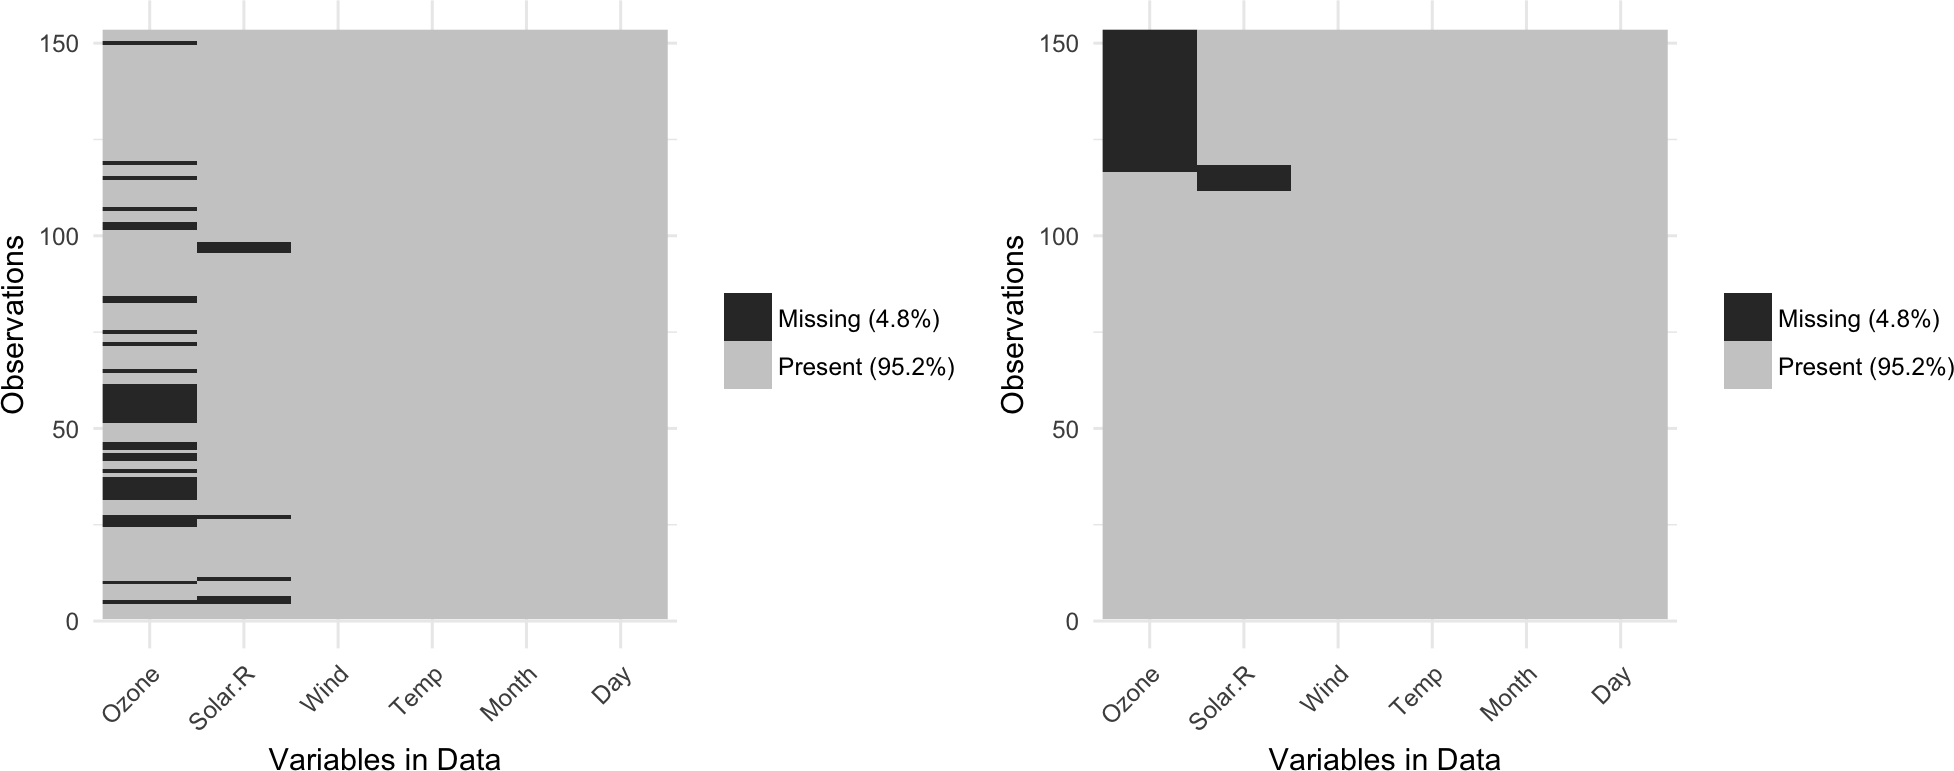
\includegraphics{jsm2017_files/figure-latex/unnamed-chunk-1-1.png}

Similar approaches has been used in other missing data packages such as
VIM, mi, Amelia, and MissingDataGUI. However this plot provides the
additional benefits of being in the ggplot framework, which gives users
greater control over the plot appearance, the interface and provides the
plot in ggplot, which allows for the user to alter and update the figure
as they need. To produce this plot, the data is required to be in long
form.

\textbf{Facetted plots}

An advantage of the wide shadow format is that it allows for referring
to missingness of other variables along the values of another variable.
For example:

\begin{Shaded}
\begin{Highlighting}[]
\KeywordTok{ggplot}\NormalTok{(}\DataTypeTok{data =} \KeywordTok{bind_shadow}\NormalTok{(airquality),}
       \KeywordTok{aes}\NormalTok{(}\DataTypeTok{x =} \NormalTok{Ozone)) +}\StringTok{ }
\StringTok{  }\KeywordTok{geom_histogram}\NormalTok{() +}\StringTok{ }
\StringTok{  }\KeywordTok{facet_wrap}\NormalTok{(~Solar.R_NA,}
             \DataTypeTok{ncol =} \DecValTok{1}\NormalTok{)}
\end{Highlighting}
\end{Shaded}

\begin{verbatim}
## `stat_bin()` using `bins = 30`. Pick better value with `binwidth`.
\end{verbatim}

\begin{verbatim}
## Warning: Removed 37 rows containing non-finite values (stat_bin).
\end{verbatim}

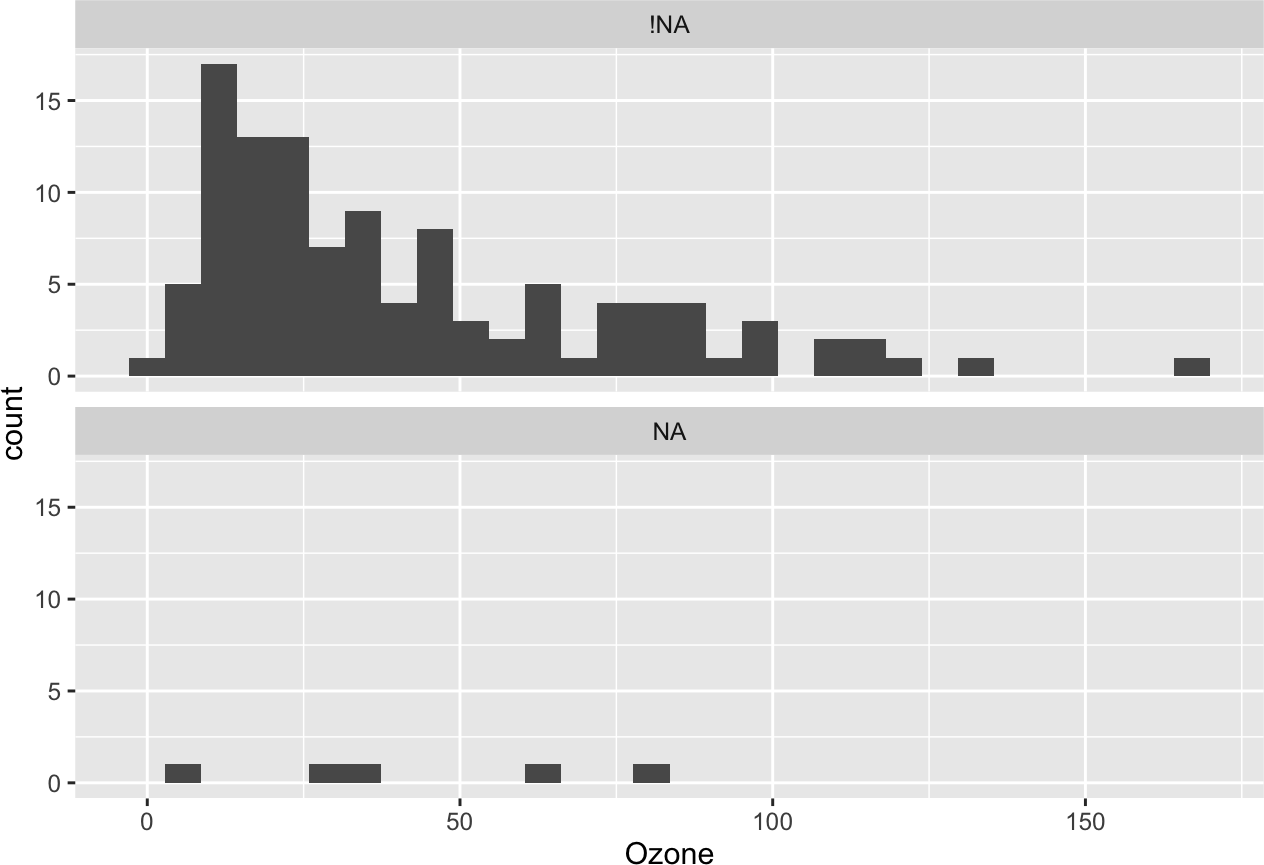
\includegraphics{jsm2017_files/figure-latex/unnamed-chunk-2-1.png}

\begin{Shaded}
\begin{Highlighting}[]
\KeywordTok{ggplot}\NormalTok{(}\DataTypeTok{data =} \KeywordTok{bind_shadow}\NormalTok{(airquality),}
       \KeywordTok{aes}\NormalTok{(}\DataTypeTok{x =} \NormalTok{Ozone,}
           \DataTypeTok{colour =} \NormalTok{Solar.R_NA)) +}\StringTok{ }
\StringTok{  }\KeywordTok{geom_density}\NormalTok{()}
\end{Highlighting}
\end{Shaded}

\begin{verbatim}
## Warning: Removed 37 rows containing non-finite values (stat_density).
\end{verbatim}

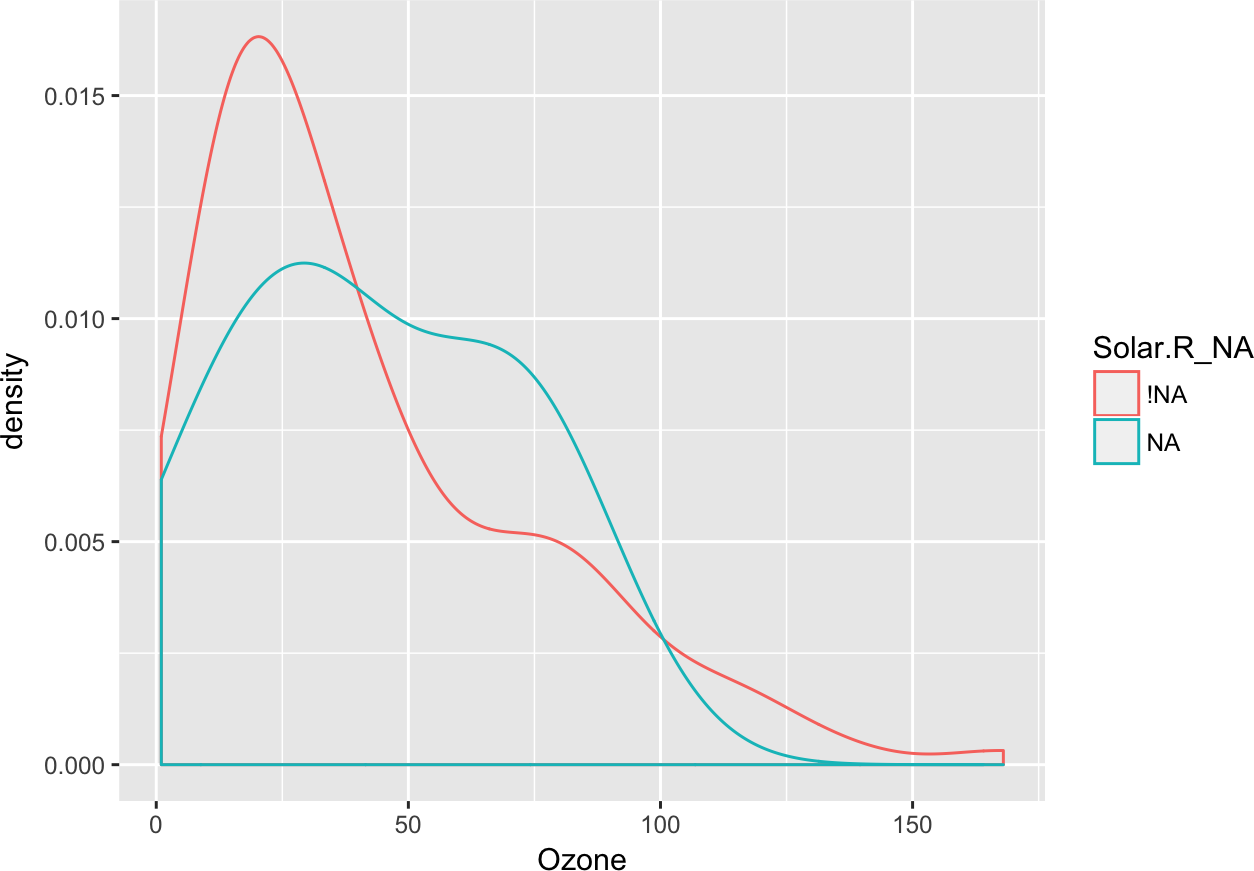
\includegraphics{jsm2017_files/figure-latex/unnamed-chunk-2-2.png}

This plot shows a histogram of Ozone, showing what the distribution of
Ozone is when Solar.R is missing.

Using this data structure facilitates missing data visualisation with
ggplot as it means that the user can directly refer to the variable that
they want to explore missingness. In the case above, the user is looking
at a histogram of Ozone, but is then able to look at how many Ozone
values are affected by Solar.R. In cases where there is no missing data
in the variable that they want to ``split'' the missingness by, the plot
simple returns a single facetted plot.

A similar method of visualisation could also be explored using
\texttt{geom\_missing\_point()} from the ggmissing package:

\begin{Shaded}
\begin{Highlighting}[]
\KeywordTok{ggplot}\NormalTok{(}\DataTypeTok{data =} \NormalTok{airquality,}
       \KeywordTok{aes}\NormalTok{(}\DataTypeTok{x =} \NormalTok{Ozone,}
           \DataTypeTok{y =} \NormalTok{Solar.R)) +}\StringTok{ }
\StringTok{  }\KeywordTok{geom_missing_point}\NormalTok{()}
\end{Highlighting}
\end{Shaded}

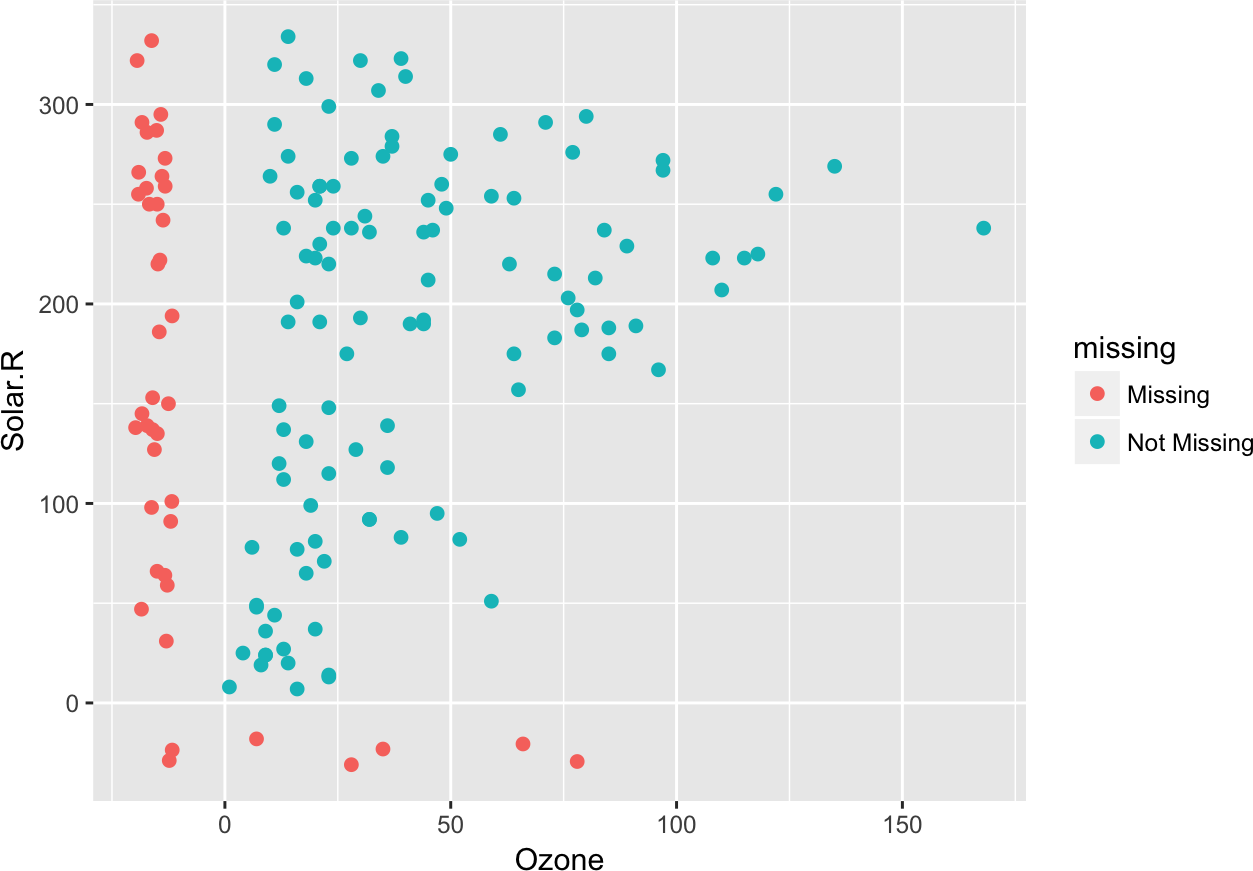
\includegraphics{jsm2017_files/figure-latex/unnamed-chunk-3-1.png}

This utilises methods from ggobi and Manet, where missing values are
replaced with values 10\% lower than the minimum value in that variable,
the missing values are also different colours, so that missingness
becomes preattentive.

\subsection{Usage}\label{usage}

Numerical summaries of missing data are also made easy with some helper
functions from the \texttt{ggmissing} package. For example, finding the
overall proportion of missing values in the data overall, or the cases,
or variables, can be done with \texttt{percent\_missing\_*} functions.

Single number summaries:

\begin{itemize}
\tightlist
\item
  The proportion elements in dataset that contains missing values
\item
  The proportion of variables that contain any missing values
\item
  the proportion of cases that contain any missing values
\end{itemize}

\begin{Shaded}
\begin{Highlighting}[]
\KeywordTok{percent_missing_df}\NormalTok{(airquality)}
\end{Highlighting}
\end{Shaded}

\begin{verbatim}
## [1] 4.793028
\end{verbatim}

\begin{Shaded}
\begin{Highlighting}[]
\KeywordTok{percent_missing_var}\NormalTok{(airquality)}
\end{Highlighting}
\end{Shaded}

\begin{verbatim}
## [1] 33.33333
\end{verbatim}

\begin{Shaded}
\begin{Highlighting}[]
\KeywordTok{percent_missing_case}\NormalTok{(airquality)}
\end{Highlighting}
\end{Shaded}

\begin{verbatim}
## [1] 27.45098
\end{verbatim}

We can also look at the number and percent of missings in each case, and
in each variable with \texttt{summary\_missing\_case}, and
\texttt{summary\_missing\_var}, which both return tibbles.

\begin{Shaded}
\begin{Highlighting}[]
\NormalTok{ggmissing::}\KeywordTok{summary_missing_case}\NormalTok{(airquality)}
\end{Highlighting}
\end{Shaded}

\begin{verbatim}
## # A tibble: 153 × 3
##     case n_missing  percent
##    <int>     <int>    <dbl>
## 1      1         0  0.00000
## 2      2         0  0.00000
## 3      3         0  0.00000
## 4      4         0  0.00000
## 5      5         2 33.33333
## 6      6         1 16.66667
## 7      7         0  0.00000
## 8      8         0  0.00000
## 9      9         0  0.00000
## 10    10         1 16.66667
## # ... with 143 more rows
\end{verbatim}

\begin{Shaded}
\begin{Highlighting}[]
\NormalTok{ggmissing::}\KeywordTok{summary_missing_var}\NormalTok{(airquality)}
\end{Highlighting}
\end{Shaded}

\begin{verbatim}
## # A tibble: 6 × 3
##   variable n_missing   percent
##      <chr>     <int>     <dbl>
## 1    Ozone        37 24.183007
## 2  Solar.R         7  4.575163
## 3     Wind         0  0.000000
## 4     Temp         0  0.000000
## 5    Month         0  0.000000
## 6      Day         0  0.000000
\end{verbatim}

We can also present tabulations that present more complicated inferences
with \texttt{table\_missing\_case} and \texttt{table\_missing\_var}.
These tally up the number of missings in each case or variable, then
describe how many cases or variables have that many missings, and the
percentage of

\begin{Shaded}
\begin{Highlighting}[]
\NormalTok{ggmissing::}\KeywordTok{table_missing_case}\NormalTok{(airquality)}
\end{Highlighting}
\end{Shaded}

\begin{verbatim}
## # A tibble: 3 × 3
##   n_missing_in_case n_cases  percent
##               <int>   <int>    <dbl>
## 1                 0     111 72.54902
## 2                 1      40 26.14379
## 3                 2       2  1.30719
\end{verbatim}

\begin{Shaded}
\begin{Highlighting}[]
\NormalTok{ggmissing::}\KeywordTok{table_missing_var}\NormalTok{(airquality)}
\end{Highlighting}
\end{Shaded}

\begin{verbatim}
## # A tibble: 3 × 3
##   n_missing_in_var n_vars   percent
##              <int>  <int>     <dbl>
## 1                0      4 2.6143791
## 2                7      1 0.6535948
## 3               37      1 0.6535948
\end{verbatim}

\section{Discussion}\label{discussion}

Here we have discussed some of the common issues with investigating
missing data.

You can also write a few sentences on computing on the fly vs data
storage

Limitation

\begin{itemize}
\item
  We didn't discuss how to visualise imputations, but you can imagine a
  similar framework for labelling imputations in a data structure.
\item
\end{itemize}

Future work explore model-based approaches for exploring based missing
data structures.

\section{References}\label{references}


\end{document}
